\begin{figure}
\begin{tabular}{@{}c@{}c@{}c@{}}
\begin{subfigure}[b]{0.30\textwidth}
\begin{center}
{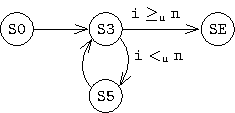
\includegraphics[scale=1.15]{chapters/figures/figMallocSpecCfg.pdf}}
\end{center}
\vspace{17px}
\caption{\label{figrr:llAllocSpecIRCFG}CFG of \SpecL{} procedure}
\end{subfigure}%
&
\begin{subfigure}[b]{0.30\textwidth}
\begin{center}
{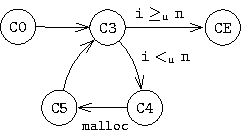
\includegraphics[scale=1.1]{chapters/figures/figMallocCCfg.pdf}}
\end{center}
\vspace{5px}
\caption{\label{figrr:llAllocCCFG}CFG of C procedure}
\end{subfigure}%
&
\begin{subfigure}[b]{0.40\textwidth}
\begin{center}
{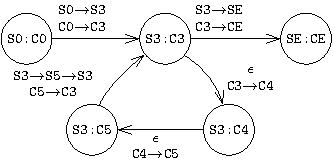
\includegraphics[scale=1.1]{chapters/figures/figMallocProductCfg.pdf}}
\end{center}
\caption{\label{figrr:llAllocProductCFG}Product-CFG}
\end{subfigure}%
\\
\end{tabular}
\caption{\label{figrr:llAllocAllCFGs}\Cref{figrr:llAllocSpecIRCFG,figrr:llAllocCCFG} shows the CFG representation of \SpecL{} and C IRs in \cref{figr:llAllocSpecIR,figr:llAllocCIR}
for the {\tt mk\_list} procedures in \cref{fig:llAllocSpec,fig:llAllocC}.
The product-CFG representing path correlations between \cref{figrr:llAllocSpecIRCFG,figrr:llAllocCCFG} is shown in \cref{figrr:llAllocProductCFG}.}
\end{figure}